\documentclass{article}
\usepackage{german}

\setlength{\emergencystretch}{15pt}

\usepackage{graphicx}

\usepackage{amsmath}

\begin{document}

\section{Herleitung}

\subsection{Methode}
\paragraph{Start}
$z_k^{(i)} = x;z_k^{(i+1)} = y$ in die Weierstraß-Iteration einsetzen 
\begin{equation}
    g(x) = y = x - \frac{p(x)}{\prod_{j=1;j\neq k}^{n} (x-z_j^{(i)})}
\end{equation}
Graph angucken (Beispiel)
\begin{figure}[h]
    \centering
    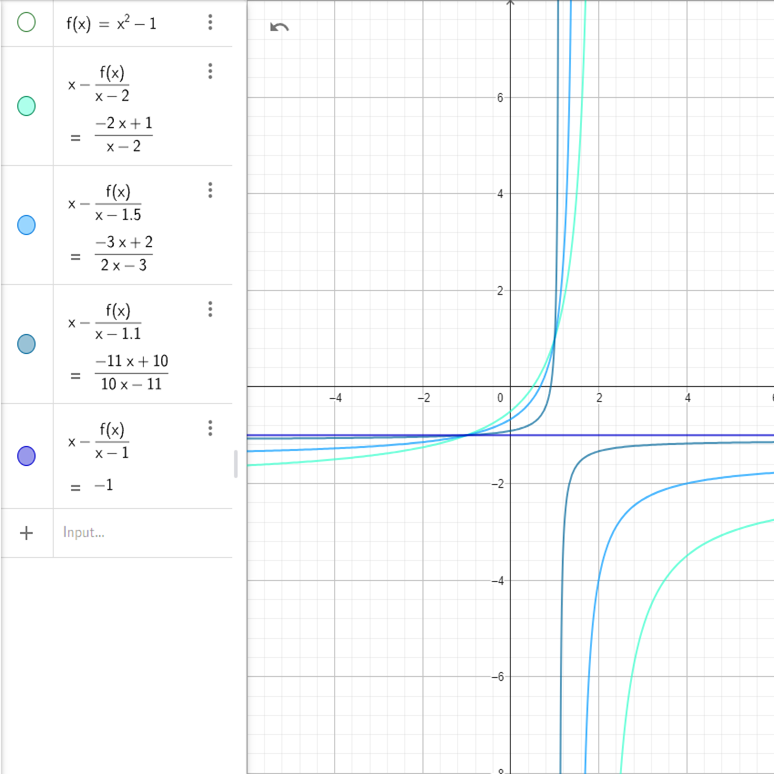
\includegraphics[scale=.6]{BeispielHerleitung.png}
    \caption{Beispiel: $x^2-1$ für die Nullstelle $-1$}
\end{figure}
%-------------------------------------------------------------------------------------------------------------------
\paragraph{Wenn alle Nullstellen gefunden konstant} Irrelevant
Falls die restlichen Nullstellen gefunden wurden waagrechte Gerade -> Für jeden Wert $z_k^(i)$ kommt die Nullstelle $z_k$ raus
Nicht zu beachten, da die exakte Nullstelle erst im unendlichen gefundne wird
\begin{align*}
    y &= x - \frac{p(x)}{\prod_{j=1;j\neq k}^{n} (x-z_j)} \\
    &= x - (x-z_k) \\
    &= z_k
\end{align*}
%-------------------------------------------------------------------------------------------------------------------
\paragraph{Nicht der Fall}
Sonst gebrochen rationale Funktion
%-------------------------------------------------------------------------------------------------------------------
\paragraph{Vergleich mit waagrechten}
Diese verläuft ähnlich die die waagrechte, allerdings hat Definitionslücken und ist um diese \glqq verfälscht\grqq. Diese \glqq Verfälschung\grqq\space nimmt mit steigendem Abstand zu der Definitionslücke ab, da der gebrochene Term der Funktion immer kleiner wird. 
$g(z_k) = z_k$
%-------------------------------------------------------------------------------------------------------------------
\paragraph{$z_k$ positiv}

%-------------------------------------------------------------------------------------------------------------------
\paragraph{$z_k$ negativ}
%-------------------------------------------------------------------------------------------------------------------
\paragraph{Verhalten nicht auf der Nullstelle}
Mit jeder iteration näher an die Nullstlle
%-------------------------------------------------------------------------------------------------------------------
\paragraph{verhalten auf der Nullstelle}
$g(z_k) = z_k$ -> Bleibt stehen -> Nullstelle gefunden
%-------------------------------------------------------------------------------------------------------------------
\paragraph{Außnahmen und Probleme}
Definitionslücken




\end{document}